\begin{definefigure}{fig:platform}
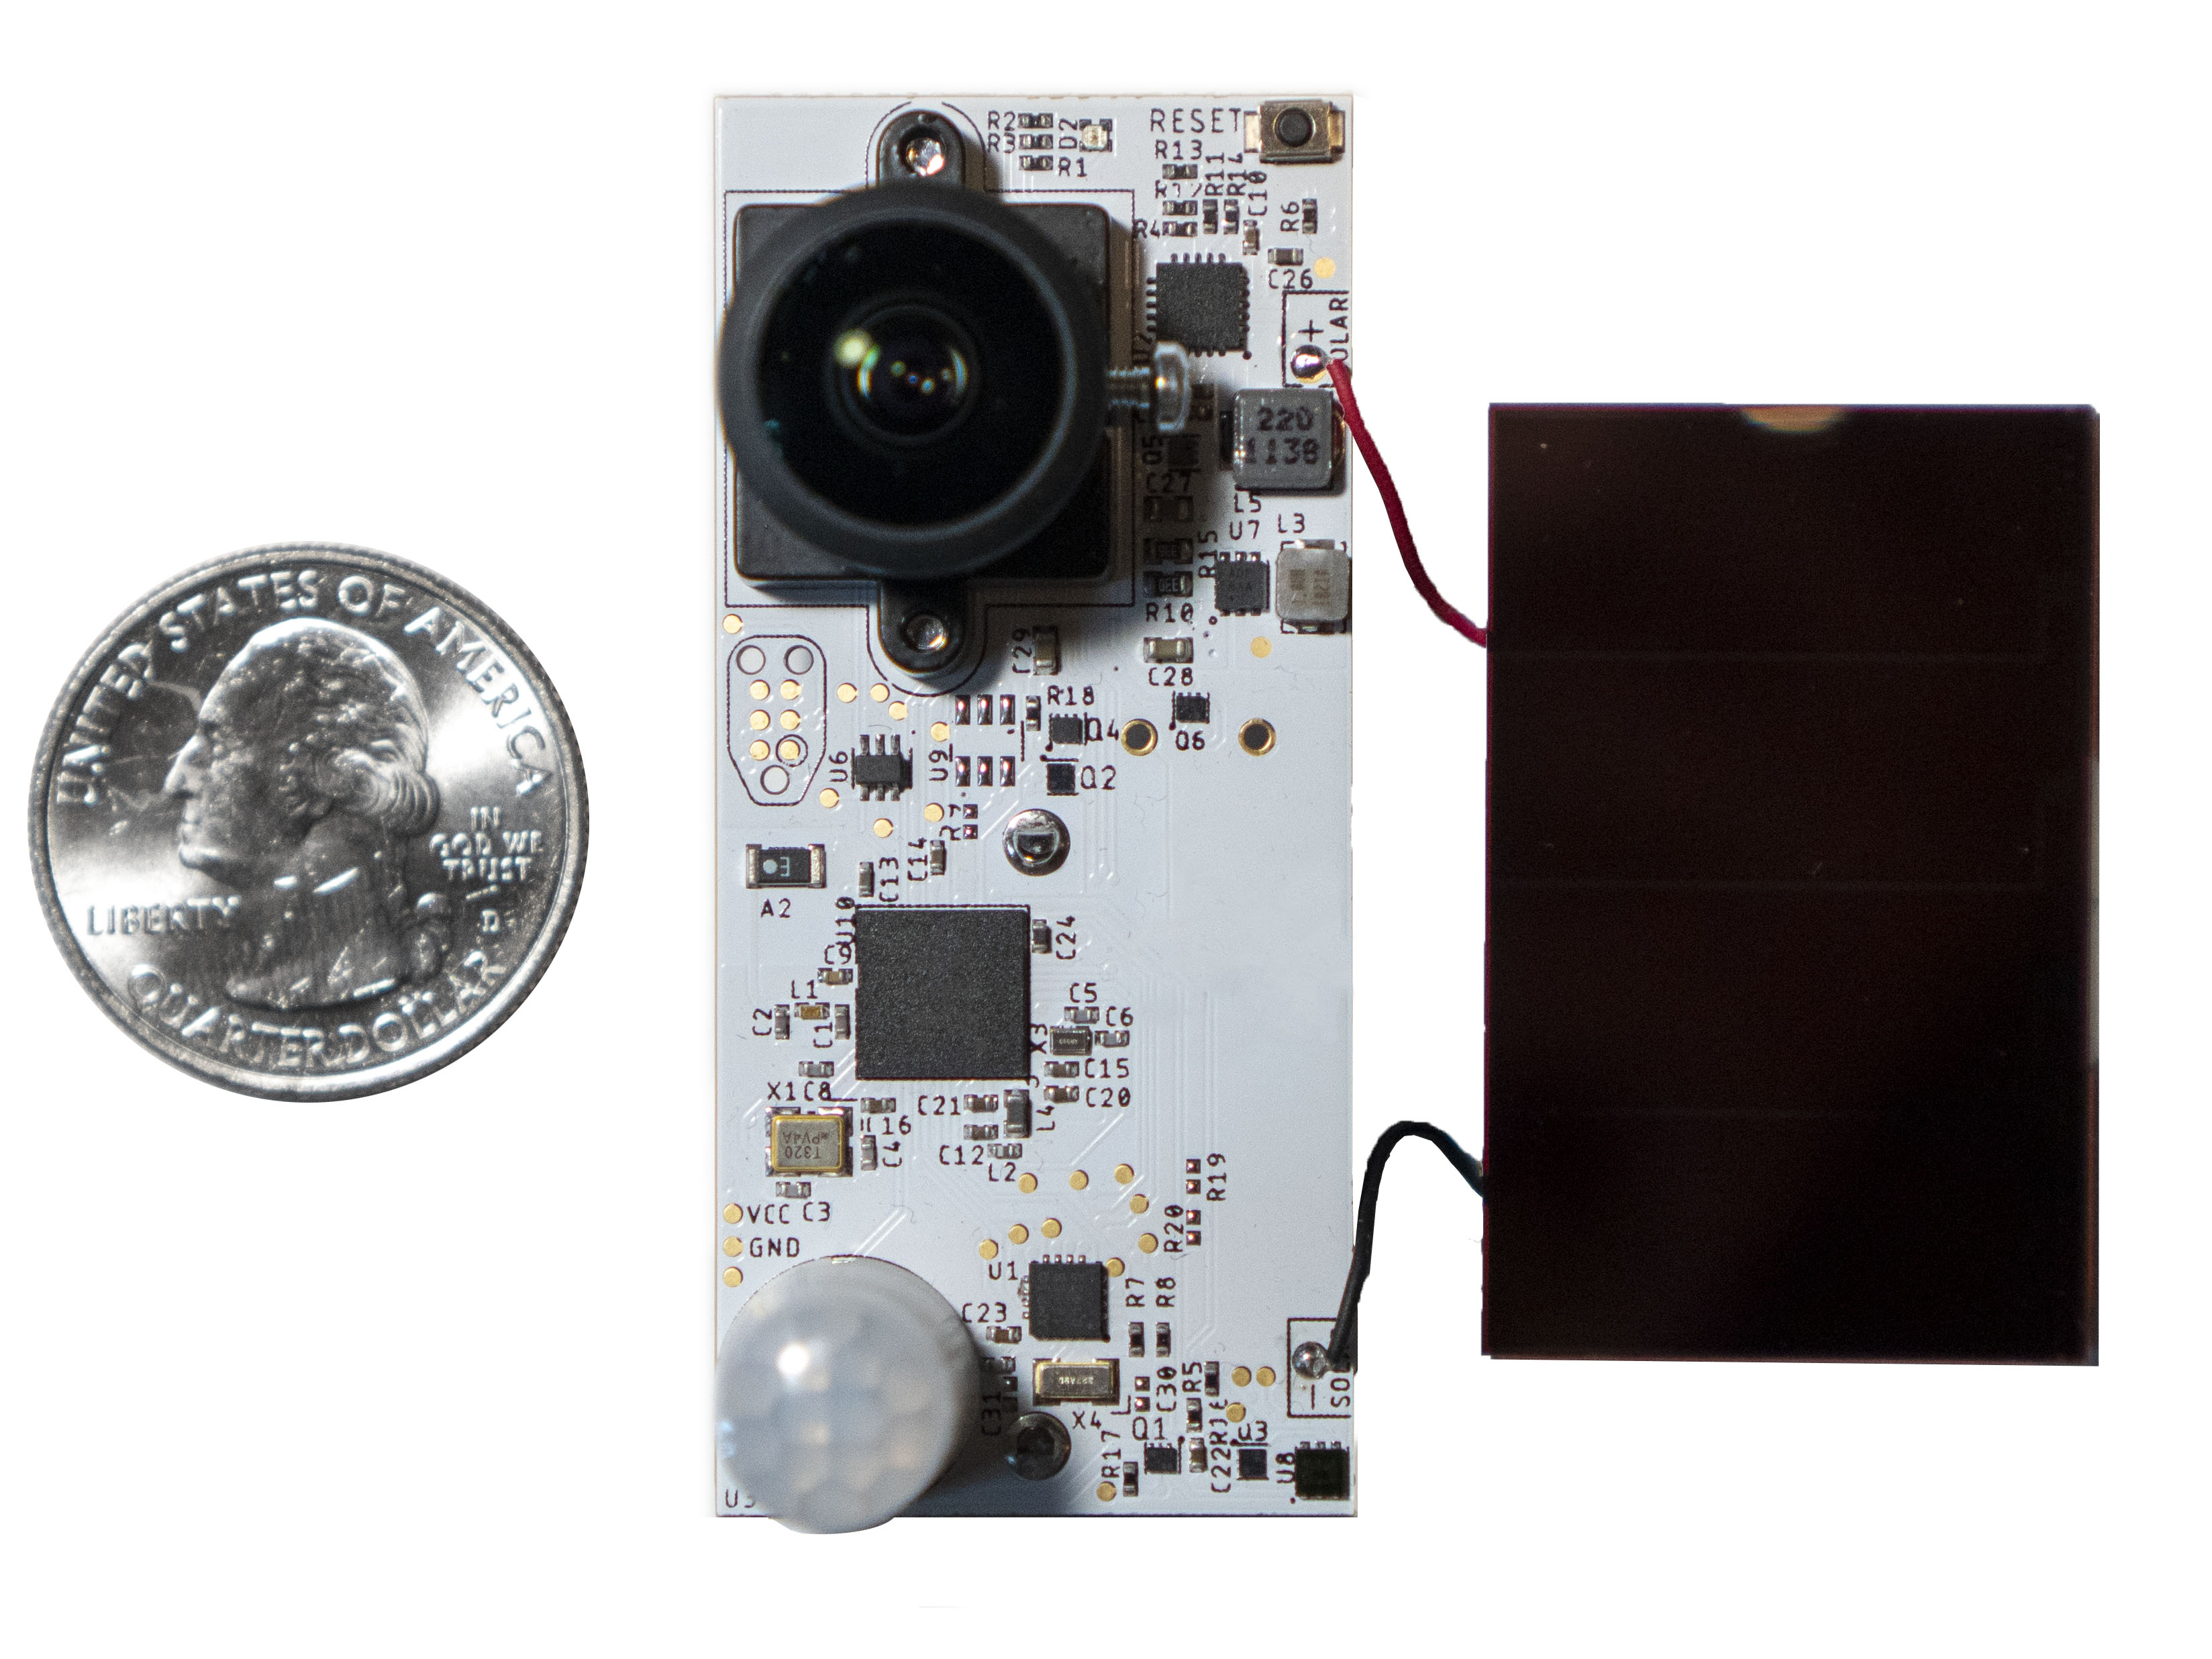
\includegraphics[width=\columnwidth]{images/platform_quarter.jpg}
\vspace{-2\baselineskip}
\caption{ \name{}. 
    \normalfont{A wireless camera platform for indoor computer vision applications. To achieve a multi-year lifetime, we employ energy harvesting with a photo-voltaic panel. A quarter is included for scale. \name is capable of local inference as well as full image transmission to cloud image processing pipelines. The platform is 10\,mm thick, and has a rechargeable and non-rechargeable battery on its backside}
}
\end{definefigure}
\placefigure{fig:platform}

\section{Introduction}
Image inference, including classification and object detection, has been one of the most active areas of computer science and machine learning research. However, due to the cost and difficulty of deploying wired cameras, applications based on continuous image sensing is untenable. This is especially true for indoor applications, where camera density must be higher for sufficient coverage.

Indoor wireless camera sensors have been heavily researched and commercialized over the past fifteen years, but due to the technology available at the time, as well as incompatibilities between design decisions and longevity, these platforms are typically limited to lifetimes of at most weeks to months~\cite{rowe2007firefly,rahimi2005cyclops,blinkindoor,wyzeoutdoor,josephson2019wireless}. 
Deployment of these platforms beyond small or temporary installations remain a challenge due to the cost of frequent battery replacement.
With the confluence of new and improved COTS technology, like low power processors, radios, and image sensors, it is worth revisiting the design of wireless camera sensors. 

Recent improvements in microcontrollers go beyond lower power \cite{kim2018system}. Processors now include hardware floating point support, single cycle multiplies, and data-parallel instruction (SIMD) support. The promise of new dedicated accelerators provides the potential of significant improvements in inference performance on low power systems~\cite{armm55,himaxwiseeye}. This has led to renewed interest in performing complex local inference on a battery budget, especially as transmitting large data like images is traditionally very expensive. However, radios have also become far more power efficient, which again muddies the conventional wisdom. Indeed, it is now much cheaper to transmit large data to a more capable system. Desktop or server class machines handily outclass their low power microcontroller and accelerator brethren on performance, providing the ability to perform more complex and accurate inference, if only data can be efficiently delivered to them.
%Regardless of recent improvements, microcontroller and accelerator performance will continue to pale in comparison to desktop and server class computing systems. 
This is especially true as memory has not scaled at the same pace as processing.
This rapidly changing design space points to a requirement for a flexible architecture and framework for thinking about what applications are most suited for local processing versus cloud offload.
% or data transmission.

In this work, we present \name, the first wireless, energy-harvesting camera platform capable of capturing and transmitting an image every ten minutes for half a decade in indoor environments.
\name represents a culmination of recent work on low power camera sensors~\cite{josephson2019wireless,nardello2019camaroptera,naderiparizi2015wispcam} and energy harvesting sensor platforms~\cite{jackson2019capacity}. \name features a hierarchical energy harvesting system that couples a small rechargeable battery with a backup non-rechargeable battery. This combination provides the system with a long and reliable lifetime. The longevity and reliability of the platform make it suitable for long-term, low-maintenance deployments. Images captured by \name are capable of driving applications based on object detection, like people counting or interaction tracking. With default, pretrained weights, an object detection model is able to detect a person in \name images from 20 meters away.

\name is capable of performing both local inference and transmitting full images end-to-end to more powerful systems. Local inference potentially requires less energy than image transmission, and also provides significantly better privacy guarantees. In cases where privacy is not as much of a concern, image transmission to a more capable endpoint increases the flexibility and performance of inference run on images. Privacy can still be guaranteed if images are transmitted only within a local network.
We examine the implications of both architectural choices with respect to capability, energy, and latency.

Our results show that on modern SoCs, transmitting images surprisingly enables longer lifetimes and improved inference. While this conclusion is unique to indoor wireless camera sensors 
whose footprints are not dominated by their energy harvester or storage, its general methodology can be applied to other application spaces as well.
%
Through this conclusion, we develop an end-to-end architecture that makes images captured by \name accessible to data collectors and application builders. \name provides a scalable and easily deployable method to quickly gather visual data for machine learning training or datasets. Images collected by \name are easily integrated into popular computer vision and machine learning frameworks like OpenCV, TensorFlow, and PyTorch. Using these tools, high level applications can be built to drive visual applications like building occupancy counting for more efficient energy management and critical infrastructure monitoring atop a long-lived deployment of wireless \name devices.

%Additionally, privacy is a serious concern, and we demonstrate that \name is capable of some local inference. In cases where applications require capability over privacy, images can be transmitted end-to-end to the cloud, or to a more local endpoint. 
%This provides the option to still maintain some privacy when transmitting images.



